% !TEX root = ../patchEmbeddings_review.tex

\section{Introduction}\label{sec:intro}

\emph{Instance segmentation} is a task of computer vision consisting in assigning each pixel of an image to an object instance. %, where the number of instances is usually not known in advance. 
% The most success in instance segmentation (IS) has been achieved by applying deep learning. %\cite{he2017mask,romera2016recurrent,liu2018affinity}. 
There are two main types of successful deep learning approaches to instance segmentation: proposal-based and proposal-free methods. 
Proposal-based methods consist of two steps: object detection, for example by finding bounding boxes, and assigning pixels to the detected objects. These approaches have proven to be highly successful in instance segmentation competitions like MS COCO \cite{lin2014microsoft} and CityScapes \cite{cordts2016cityscapes}. 
On the other hand, proposal-free methods adopt a bottom-up approach by directly grouping pixels into instances. Recently, there has been a growing interest for such methods that do not involve object detection, since, in certain types of data, for example microscopy images of neurons \cite{arganda2015crowdsourcing}, object instances cannot be approximated by bounding boxes and are usually larger than the field of view of the deep learning model. 
% More motivation: They are at the same time limited by the quality of the object detection routine, which is hard to train on small datasets (but no ref for this)

In this work, we focus on a proposal-free method, where a Convolutional Neural Network (CNN) is trained to predict, for every pixel $i$ in the image, a patch of fixed size representing the binary mask of the instance object to which pixel $i$ belongs. The probability mask predicted in each patch is centered at the corresponding pixel $i$ and represents then a dense local neighborhood structure of pixel $i$. Whenever the object instance associated to $i$ is bigger than the size of the patch, only a partial probability mask of the object is predicted. 
% In the following, we will call these masks as \patch or LSPM.

A naive way to predict one $N\times N$ \patch  for each pixel in an image would be to use a fully convolutional model with $N^2$ output channels, where each channel represents a pixel of the corresponding mask. However, depending on the size of the predicted masks, this approach would become unfeasible and extremely memory-consuming.

Our first contribution is a fully convolutional model that predicts, for every pixel $i$, a representation of the associated $i$-th self-probability mask in a lower dimensional space (see Fig. \ref{fig:main_figure}). This is possible due to the fact that, among all possible neighborhood structures represented by local self-probability masks, only few of them are associated to occurring ground truth binary masks. Thus, the information included in the predicted self-probability masks can easily be encoded in a lower dimensional latent space. 

A very similar approach has been recently proposed in concurrent (currently unpublished) work \cite{hirsch2020patchperpix}, where it has been applied to the BBBC010 benchmark microscopy dataset of \emph{C. elegans} worms. In this paper, we propose a more efficient model and apply it to large 3D electron microscopy image volumes of neuron tissue in order to perform neuron segmentation. 
\emph{We compare its performances to the commonly used instance segmentation method of predicting, for each pixel, a small set of sparse short- and long-range neighborhood relations, i.e. affinities representing how likely it is for a pair of pixels to belong to the same object instance (see Fig. \ref{fig:main_figure} for a visual comparison).}
% \cite{liu2018affinity,wolf2018mutex} etc
% it achieves competitive performance on CityScapes and the challenging CREMI 2016 segmentation benchmark.

As a second contribution, we propose two distinct ways of converting the predicted per-pixel self-probability masks into edge weights of a graph representing the image, so that each node corresponds to a pixel and a graph clustering algorithm is used to obtain the final instance segmentation.
One of the two methods results in a pipeline that is as efficient as the currently winning method of the CREMI challenge \emph{(more efficient actually, because of LMC...), but achieves better accuracies and, as our results shows, outputs more consistent neighborhood structures...}.
The second proposed method yields a parameter-free algorithm achieving competitive performances, yada yada yada... 

\begin{figure}[t]
\centering
        % \includegraphics[width=0.4\textwidth,trim=0.25in 0.25in 0.68in 0.36in,clip]{./figs/SSBM_experiments.pdf} % 0.45
        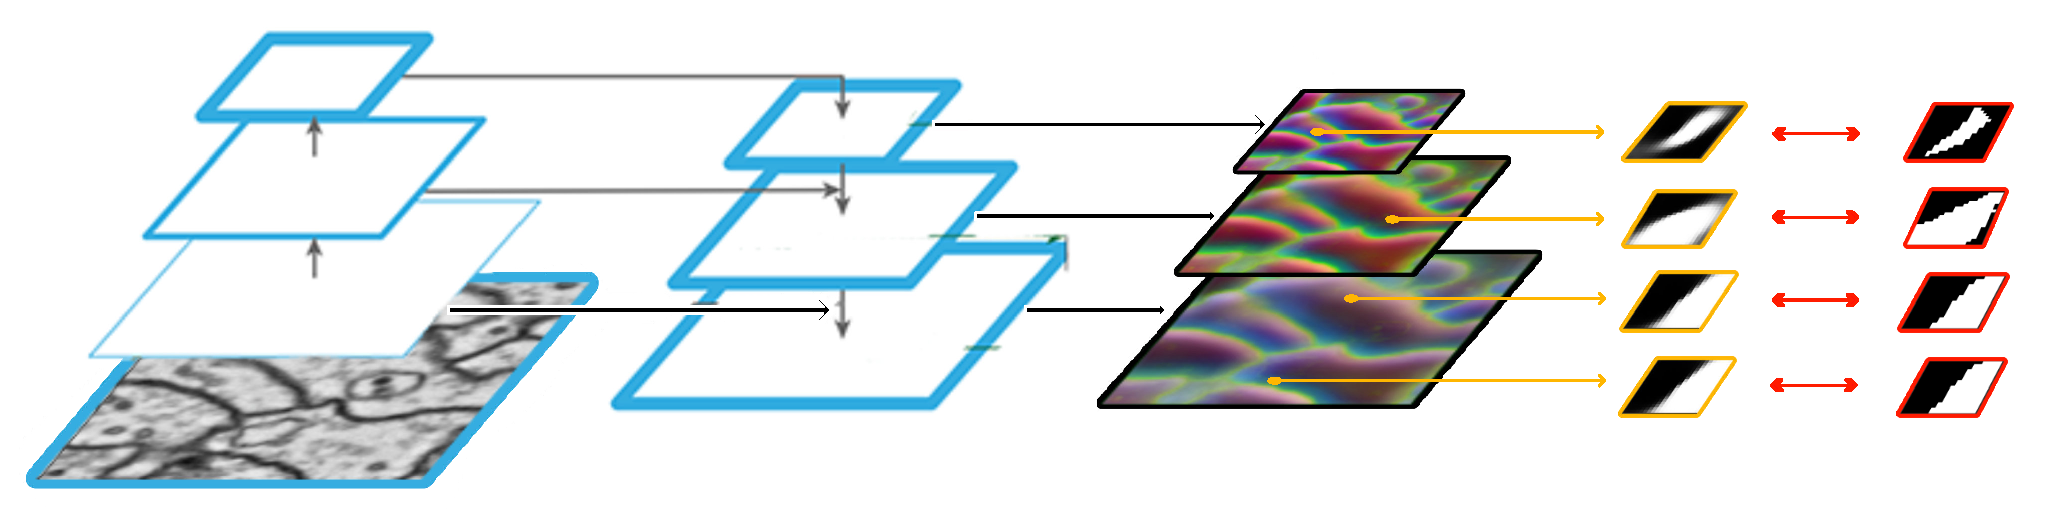
\includegraphics[width=\textwidth]{./figs/main_image.pdf} % 0.45
        \caption{Illustration of the proposed pipeline...}
    \label{fig:alg_explained}
\end{figure}


